\documentclass[11pt, oneside]{article}   	
\usepackage{geometry}                		
\geometry{letterpaper}                   		
\usepackage{graphicx}													
\usepackage{amsmath}

\title{Notes on Coalescent Theory}
\author{Patrick Barry}
						

\begin{document}
\maketitle
\section*{Chapter 1}
\begin{itemize}
\item{} Mutations give rise to all genetic polymorphisms so sampled DNA sequences 
originate from a common sequence. 
\item{} The relationship of sampled sequences can be represented by a genealogy.
\item{} When two lineages come together they are said to have coalesced. 
\item{} Within a species these gene genealogies are influenced heavily by drift.
\end{itemize} 

When we talk about genealogies some terminology is useful. Each tree will end in 
$n$ leaves which are the sequences (lineages) sampled. The branches 
will come together in a coalescent event at a vertex or node. There will be 
For any genealogy there will be $n-1$ coalescent events or vertices. The total number
of branches will be $2n-3$ if the tree is unrooted and $2n-2$ for a rooted tree. There 
will obviously be $n$ leaves or external branches so there will be $n-2$ internal 
branches. 

\begin{itemize}
\item{} \textit{Compatibility} deals with genealogies and mutational histories. 
\item{} Can be checked using the 'four-gamete' test.
	\subitem{} Subset of sample. If both subsets of one site overlap with
	\textbf{both} subsets of another site they are incompatible. A site can
	be incompatible because of incompatible genealogies or there could be
	multiple mutations on a branch.
\item{}Deal with two types of data: allele based models and nucleotide sequence models.
\item{} \textbf{Infinite-allele model}: All new mutations will produce a new allele. 
\item{} \textbf{Infinite-site model}: All new mutations will occur at a new site in the sequence.
\item{} Neutral mutations will have no effect on reproductive success allowing us to 
separate the mutational process and the genealogical process.
\end{itemize} 

There are three important summary statistics: number of segregating sites, average
number of pairwise differences, and site frequencies (site frequency spectrum).
\begin{itemize}
\item{}The number of segregating sites \textit{S} is merely the number of polymorphic 
sites in the sequence being examined.
\item{} If the infinite site model holds then all mutations will occur at a new position and
the number of segregating sites will reflect the total number of mutations that have occurred. 
\item{} The average number of pairwise differences $\pi$ is as the name suggests just an average
of the differences observed when comparing all sequences in the collection. 

\begin{equation}
\pi=\frac{1}{\binom{n}{2}}\sum_{i=1}^{n-1}\sum_{j=i+1}^{n}k_{ij}
\end{equation}
where $k_{ij}$ is the number of differences between sequences i and j. The binomial 
describes how many different comparisons can be made between n sequences. 

\item{} If we know what the ancestral base at a site is we can count the number of instances that 
a mutated base occurs as $\xi_i$.
\item{} If we do not know the ancestral base we can merely distinguish instances where one base is
present in $i$ copies and the other is present in $n-1$ copies $\eta_i$. 

\begin{equation}
\eta_i=\frac{\xi_i+\xi_{n-11}}{1+\delta_{i,n-1}}
\end{equation}
where $ \delta_{i,n-1}$ is equal to zero if $n \neq j$ and equal to 1 if $n = j$. The basic idea here is that
you don't want to double count sites when $n = j$, so you divide by 2 in those cases. 
\end{itemize}

\subsection*{Questions}
1. What is the total number of possible arrangements of the four bases (A,T,G,C) at a
single site in a sample of $n$ sequences labelled 1,2,...n?\\

If order is important, then each singe site can be occupied by 1 of 4 nucleotides. So 
the total number of arrangements would be $4^n$. However if order is unimportant
ie. $AAT=ATA=TAA$, then we need to get rid of the redundancies. In this case the total
number of arangements would be $\frac{(4+n-1)!}{n!(4-1)!}$\\

2. Draw a genealogy of a sample of six sequences, with mutations on the branches, such that
$\xi_1=1$, $\xi_2=2$, and $\xi_4=3$.\\

So $\xi_i$ is the number of sites at which the mutant base is present in $i$ copies and 
ancestral base is present in $n-i$ copies in a sample. So with the above data, we know that
we should have six sites in our sequence with one site that has one mutant base, two sites with 
two mutant bases, and three sites with four mutant sites. So let's make up some data\\

\noindent
Anct			...G...T...C...A...A...\\
Seq 1   		...A...T...C...G...G...\\
Seq 2		...G...C...C...G...G...\\	
Seq 3	  	...G...C...T...G...A...\\
Seq 4  		...G...T...T...G...A...\\
Seq 5  		...G...T...T...A...G...\\
Seq 6  		...G...T...T...A...G...\\



\begin{figure}[!htbp]
    \centering
    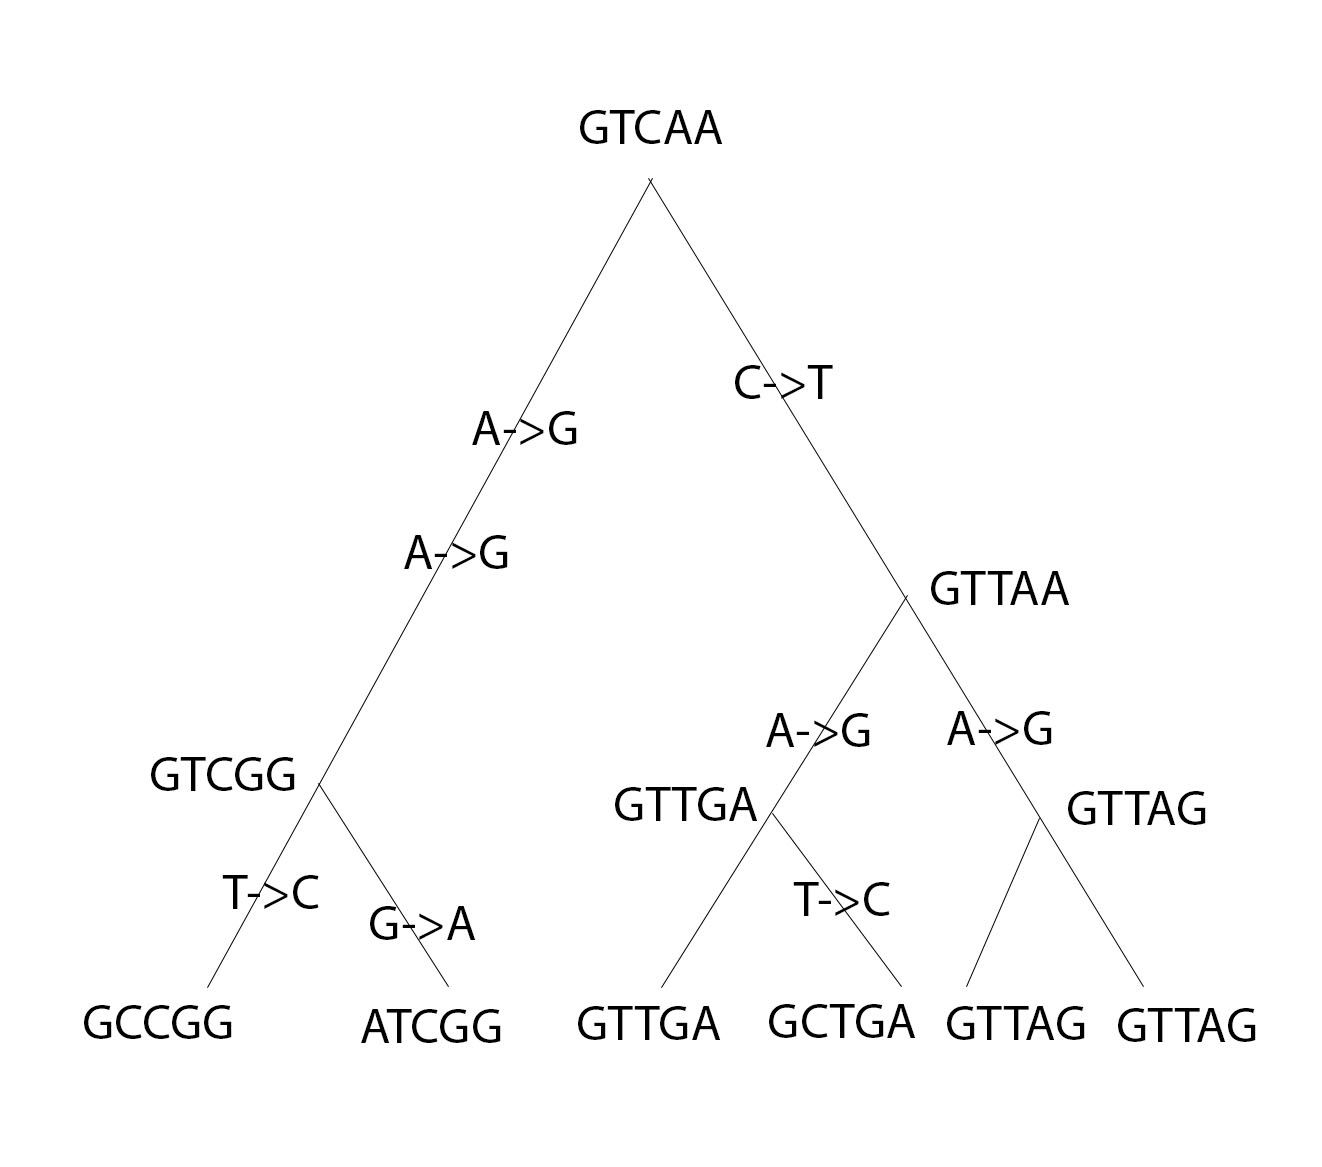
\includegraphics[width=0.8\textwidth]{./Figures/Ch1Q2.jpg}
    \caption{Geneology for $\xi_1=1$, $\xi_2=2$, and $\xi_4=3$}
    \label{fig:Ch1Q6gen}
\end{figure}




3. Do the data below pass or fail the four-gamete test? Explain your answer. \\

\noindent
Seq 1 ...A...T...G...A...\\
Seq 2 ...A...T...G...C...\\
Seq 3 ...G...T...G...A...\\
Seq 4 ...G...C...T...A...\\
Seq 5 ...G...C...G...C...\\

No, these data do not pass the four-gamete test. Sites 1 and 4 have all four possible gametes
as do sites 2 and 4. If site 4 were not sampled then the data would pass the four-gamete test. \\

4. Compute the site-frequency counts $\xi_i$,$i=1,2,3,4$, for the data above by assuming 
you have sampled an out group sequence that is identical to sequence 5. What are the folded 
site-frequency counts $\eta_i$ for these data?\\

So we can assume that the out group is sequence 5 and that we know what the ancestral states 
of each site are. Assuming the ancestral sequence is ...G...C...G...C we simply need to look at each
site and figure out how many of them have just a single copy of a mutated base ($\xi_1$), two copies ($\xi_2$), etc. We can also order the sequences with sites matching the ancestral sequences as dashes 
and mutant sites highlighted by their state change. \\

\noindent
Seq 1 AT- A\\
Seq 2 AT--\\
Seq 3 -T-A\\
Seq 4 --TA\\
Seq 5 ----\\

So the first site has two mutant copies contributing 1 to $\xi_2$. Two sites have 3 mutant copies
(sites 2 and 4) so $\xi_3=2$ and site 3 has one mutant copy making $\xi_1=1$. No site has 4 mutant
copies $\xi_4=0$. The folded site frequencies can be calculated as:\\
\begin{equation*}
\eta_1=\frac{\xi_1+\xi_{4}}{1+\delta_{1,4}}
=\frac{1+0}{1+0}=1
\end{equation*}
\begin{equation*}
\eta_2=\frac{\xi_2+\xi_{3}}{1+\delta_{2,3}}
=\frac{1+3}{1+0}=3
\end{equation*}

5. Show two different methods for computing the average number of pairwise sequence differences 
$pi$, for the data above.\\

\begin{equation*}
\pi=\frac{1}{\binom{5}{2}}\sum_{i=1}^{4}\sum_{j=i+1}^{5}k_{ij}
\end{equation*}
\begin{equation*}
\pi=\frac{1}{10}\sum_{i=1}^{4}\sum_{j=i+1}^{5}k_{ij}=\frac{1}{10}*22=2.2
\end{equation*}
\\
or 
\\
\begin{equation*}
\pi=\frac{1}{\binom{n}{2}}\sum_{i=1}^{n/2}i(n-i)\eta_i
\end{equation*}
\begin{equation*}
\pi=\frac{1}{10}\sum_{i=1}^{2}i(n-i)\eta_i
\end{equation*}
\begin{equation*}
\pi=\frac{1}{10}(1*4*1+2*3*3)=2.2
\end{equation*}

6. Draw a possible genealogy for the data in exercise 3, and show how the data might have been 
derived via mutations along the branches of the tree. \\

So we know that the data in exercise 3 do not pass the four-gamete test so we know that there
will be multiple mutations along a branch or the same site might have two mutations making the 
infinite sites model not hold. How many possible trees are there with 4 samples? 
We can compute the total number of rooted binary trees with $(2n-3)!!$. For 4 samples that would
be 105 possible tree configurations. \\

\noindent
Seq 1 ...A...T...G...A...\\
Seq 2 ...A...T...G...C...\\
Seq 3 ...G...T...G...A...\\
Seq 4 ...G...C...T...A...\\
Seq 5 ...G...C...G...C...\\

Again lets assume that Seq 5 is identical to the outgroup (as in question 4).\\


\begin{figure}[!htbp]
    \centering
    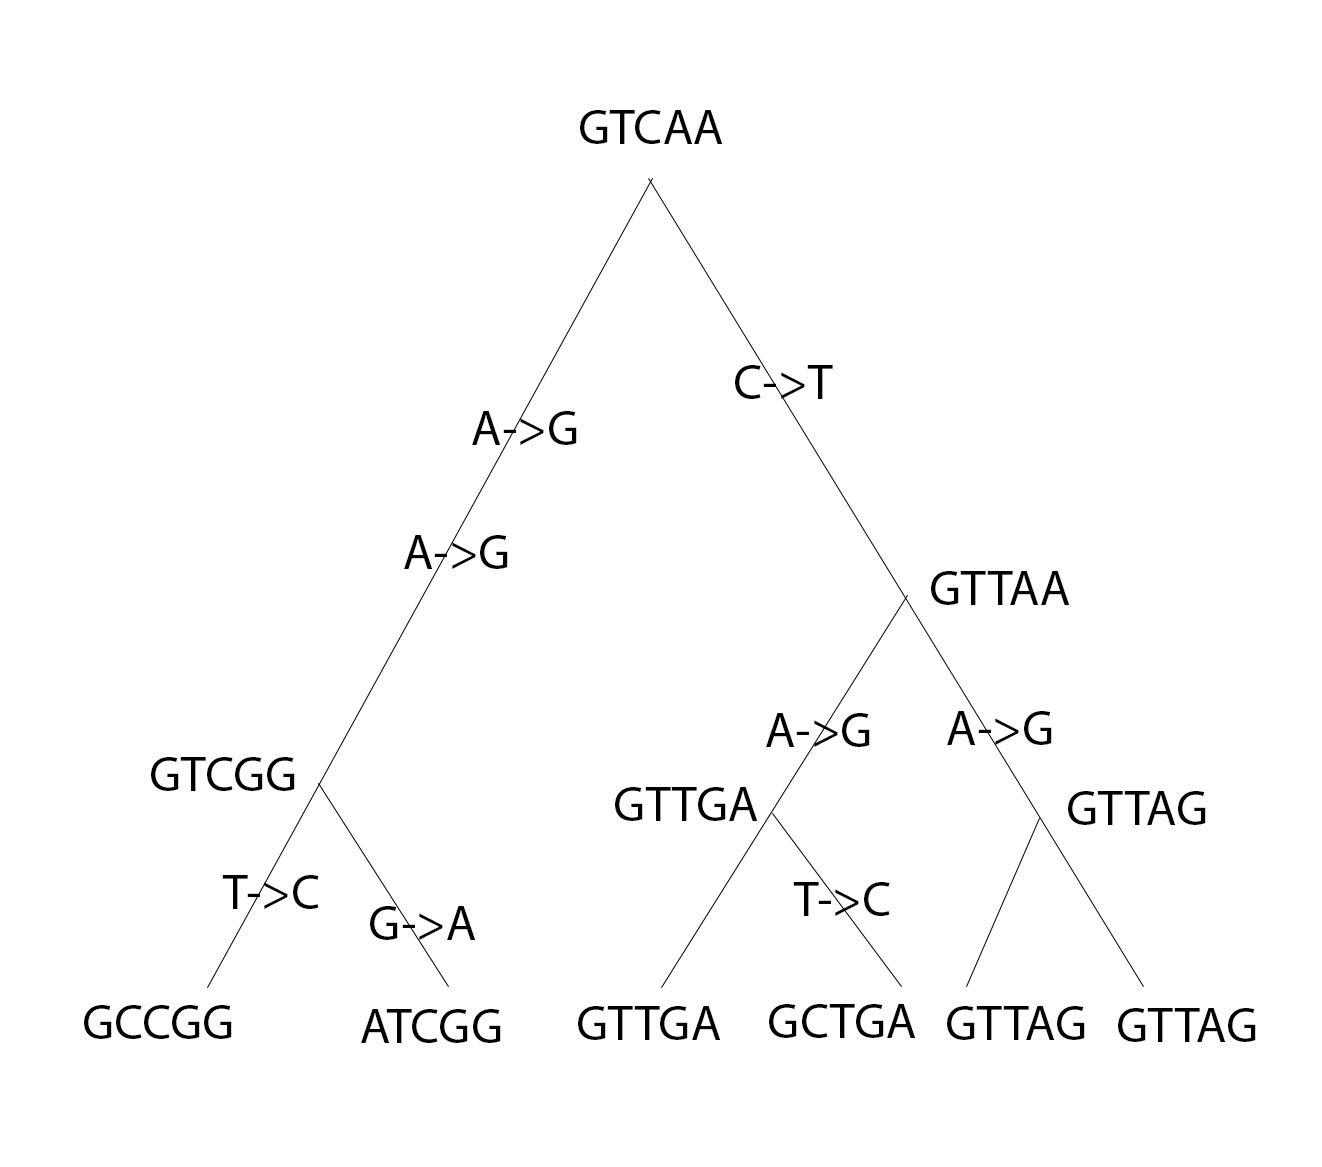
\includegraphics[width=0.8\textwidth]{./Figures/Ch1Q6.jpg}
    \caption{Geneology for data in excercise 3.}
    \label{fig:Ch1Q6gen}
\end{figure}

This is obviously just one of the many potential geneologies that could be drawn for the data
in question three.





\end{document}  